\documentclass[./main.tex]{subfiles}
\begin{document}
\chapter{Monte Carlo simulation of particle transport using GORILLA}
This chapter is taken without change from \cite{paper_gorilla}, as the author of this thesis has made contributions to this publication, appearing therefore as co-author. The content is furthermore relevant to this thesis as it gives valuable insights in the application of the code $GORILLA$.
\section{Monte Carlo evaluation of neoclassical transport coefficients, performance benchmark}
\label{sec:transport}


Evaluation of neoclassical transport coefficients using the Monte Carlo
method~\cite{boozer_monte_1981,lotz_monte_1988} is widely
used for stellarators and tokamaks with 3D perturbations of the magnetic
field~\cite{wakasa_study_2008,tribaldos_monte_2001,isaev_venusf_2006,allmaier_variance_2008,velasco_calculation_2011,satake_neoclassical_2011,pfefferle_venus-levis_2014}.
An advantage of this method in its original, full-$f$ form is the use of test particle guiding-center
orbits without requiring model simplifications needed in (more efficient) local approaches. Therefore Monte Carlo methods provide
an unbiased reference point in cases where those simplifications affect the transport such as for regimes with
significant role of the tangential magnetic drift~\cite{matsuoka_effects_2015,huang_benchmark_2017}.
An obvious disadvantage is that for realistic magnetic configurations Monte Carlo methods are CPU-intensive
with most of the CPU time spent for the integration of the guiding-center motion. The application of the proposed geometric integration method for this purpose instead of the usual Runge-Kutta method results in a visible speed-up
of the computations without significantly biasing the results.
Here, this application is made for benchmarking purposes assuming that the inaccuracies in orbit integration
which are tolerable in computations of transport coefficients are also tolerable
in global modelling of macroscopic plasma parameters.

The proposed orbit integration method is applied
within a standard Monte Carlo algorithm~\cite{boozer_monte_1981}
using the Lorentz collision model for the evaluation of the mono-energetic radial diffusion coefficient $D_{11}$.
The latter is determined via the average square deviation
of the normalized toroidal flux $s$ from its starting value $s_0$ as follows,
\be{eq:def_d11}
D_{11} = \frac{1}{2 t} \langle\left(s(t) - s_0 \right)^2\rangle.
\ee
Here, angle brackets $\langle\dots\rangle$ denote an ensemble average, $s(0)=s_0$, and the test particle tracing time $t$ is chosen to
be larger than the local distribution function relaxation time $\tau_{\rm rel}$
and smaller than the radial transport time, $t=10 \tau_{\rm rel}$.
A Monte Carlo collision operator identical to that of Ref.~\cite{boozer_monte_1981} is applied here in-between
constant collisionless orbit integration steps $\Delta t$. These steps are small enough compared to the typical bounce time
$\tau_\mathrm{b}$ and collision time $\tau_\mathrm{c}$,
\be{eq:def_time_step_MC}
\Delta t = \min \left(\frac{\tau_\mathrm{b}}{20},\frac{\tau_{\mathrm{c}}}{20} \right).
\ee
Here, $\tau_{\mathrm{c}} = 1/\nu$ and $\tau_\mathrm{b} = 2 \pi R_0 / (v N_\mathrm{tor.})$ with $\nu$,  $R_0$, $v$ and $N_\mathrm{tor}$ denoting collisional deflection frequency, major radius, particle velocity and
number of toroidal field periods, respectively. The relaxation time $\tau_{\rm rel}$ is determined as the largest of
$\tau_{\mathrm{c}}$ and $\tau_\mathrm{b}^2/\tau_{\mathrm{c}}$.

%
\begin{figure}[t]
	\centerline{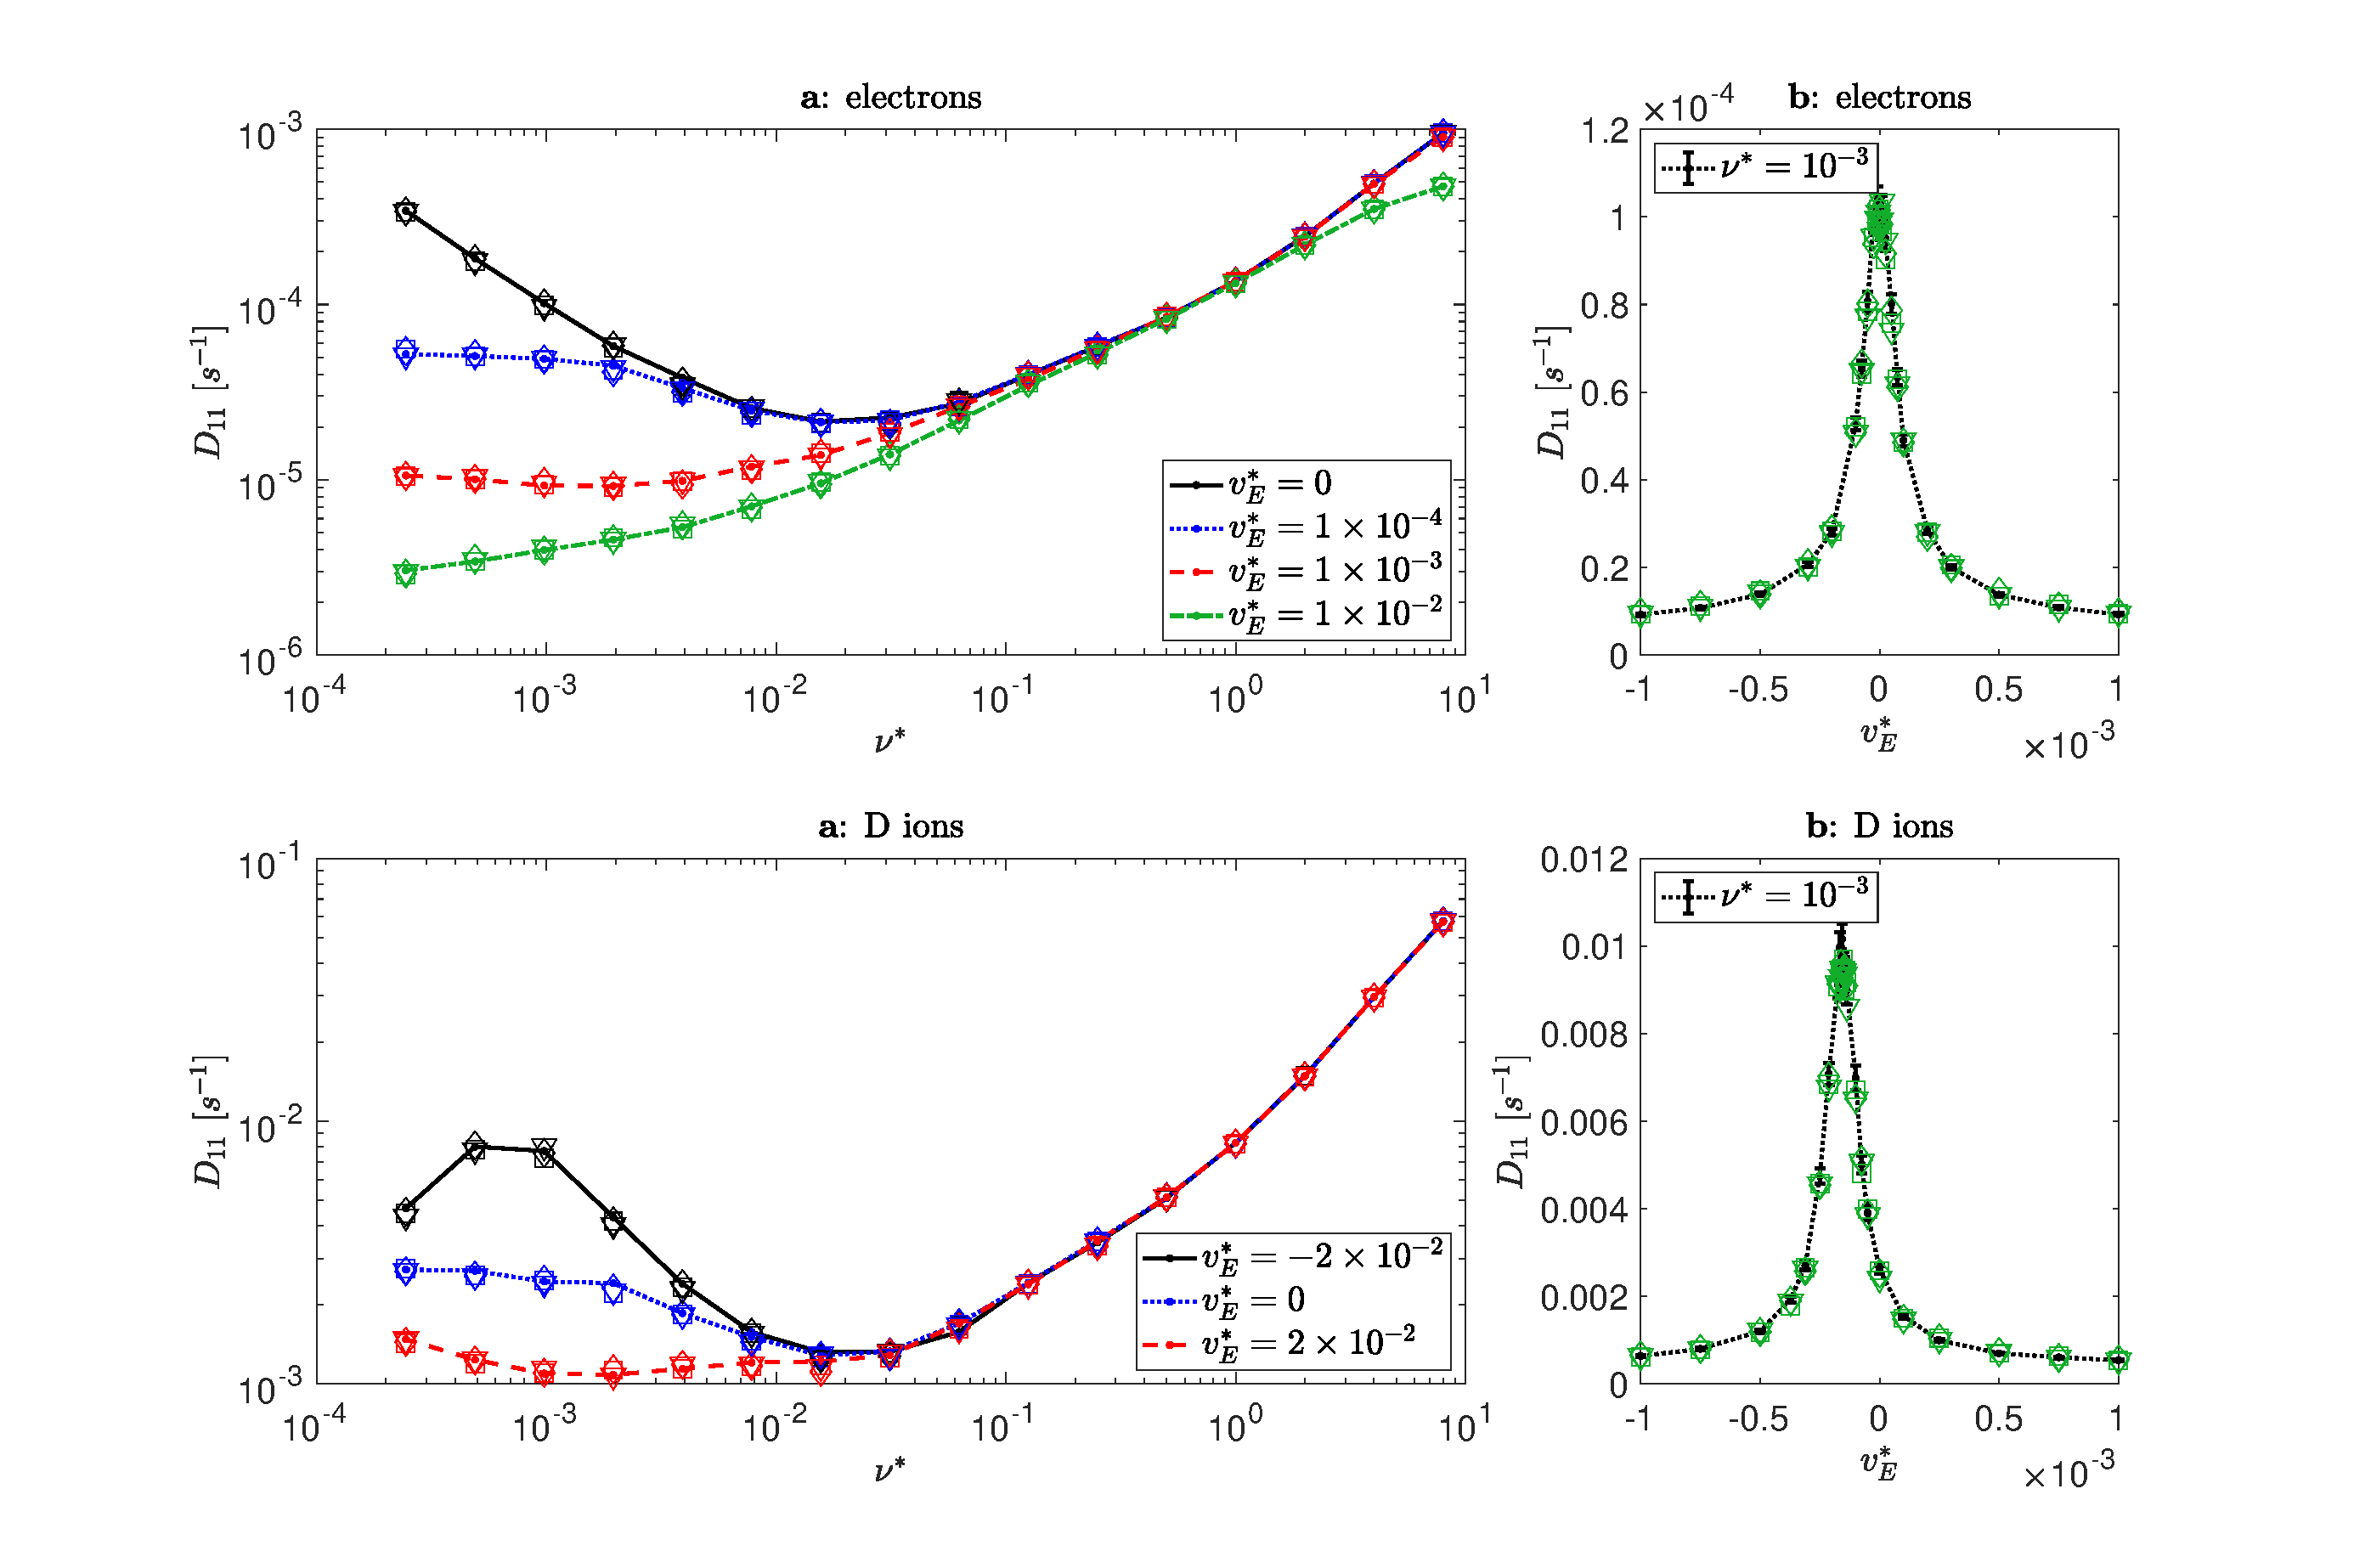
\includegraphics[keepaspectratio,width=1.1\linewidth]{figures/transport_coefficient_electrons_dions.eps}}
	\captionsetup{justification=raggedright,singlelinecheck=false,textfont=footnotesize,labelfont=footnotesize}
	\caption{Mono-energetic radial diffusion coefficients $D_{11}$ for electrons (top) and deuterium
	ions (bottom)
	as functions of (a) normalized collisionality $\nu^\ast$ and (b)  Mach number $v_E^\ast$.
	Lines of various styles (see the legends) - reference computation, markers - results of geometric
	integration with polynomial solution of the order $K$ for $K=2$ ($\Diamond$), $K=3$ ($\square$)
	and $K=4$ ($\triangledown$).
	Error bars indicate $95$~\% confidence interval.}
	\label{fig:transport_coefficient_electrons_dions}
\end{figure}
%
In the present example, the mono-energetic radial diffusion coefficient has been evaluated
for the quasi-isodynamic stellarator configuration~\cite{drevlak_quasi-isodynamic_2014}
used also for collisionless orbits in section~\textrm{III B} of \cite{paper_gorilla}.
Guiding-center orbits were computed with the geometric integration method in symmetry flux coordinates
using polynomial series solutions of various orders $K$.
The grid size $N_s \times N_\vartheta \times N_\varphi = 100 \times 60 \times 60$ was selected to be appropriate to
minimize the numerical diffusion (see the previous section.) In a reference computation, guiding-center
equations~\eq{standeqset} in symmetry flux variables with electromagnetic fields interpolated
by 3D cubic splines were integrated by an adaptive RK4/5 integrator.
In order to minimize statistical errors, computations have been performed for a large ensemble size
of $10000$ particles.

The results for $D_{11}$ computed for 3 keV electrons and ions at $s_0=0.6$ are presented in
Fig.~\ref{fig:transport_coefficient_electrons_dions}.
Values of radial electric field $E_r$ and deflection frequency $\nu$, which determine
transport regimes, are respectively characterized here by two dimensionless
parameters~\cite{beidler_benchmarking_2011}, Mach number $v_E^\ast = c E_r /(vB_0 )$ and
collisionality $\nu^\ast = (R_0 \nu)/(\iota v)$, where $\iota$ is the rotational transform.
For the ions, in addition to the $\bE\times\bB$ rotation, also the tangential magnetic drift
plays a significant role which can be seen from the shift of the $D_{11}$ maximum on $v_E^\ast$
dependence. The results of geometric integration stay in agreement
with the reference computation within the 95 \% confidence interval in all cases even for the lowest
order polynomial solution $K=2$. Therefore, as shown below, a significant gain in the computation
time can be obtained in this kind of calculations.
%

\begin{figure}[t]
	\centerline{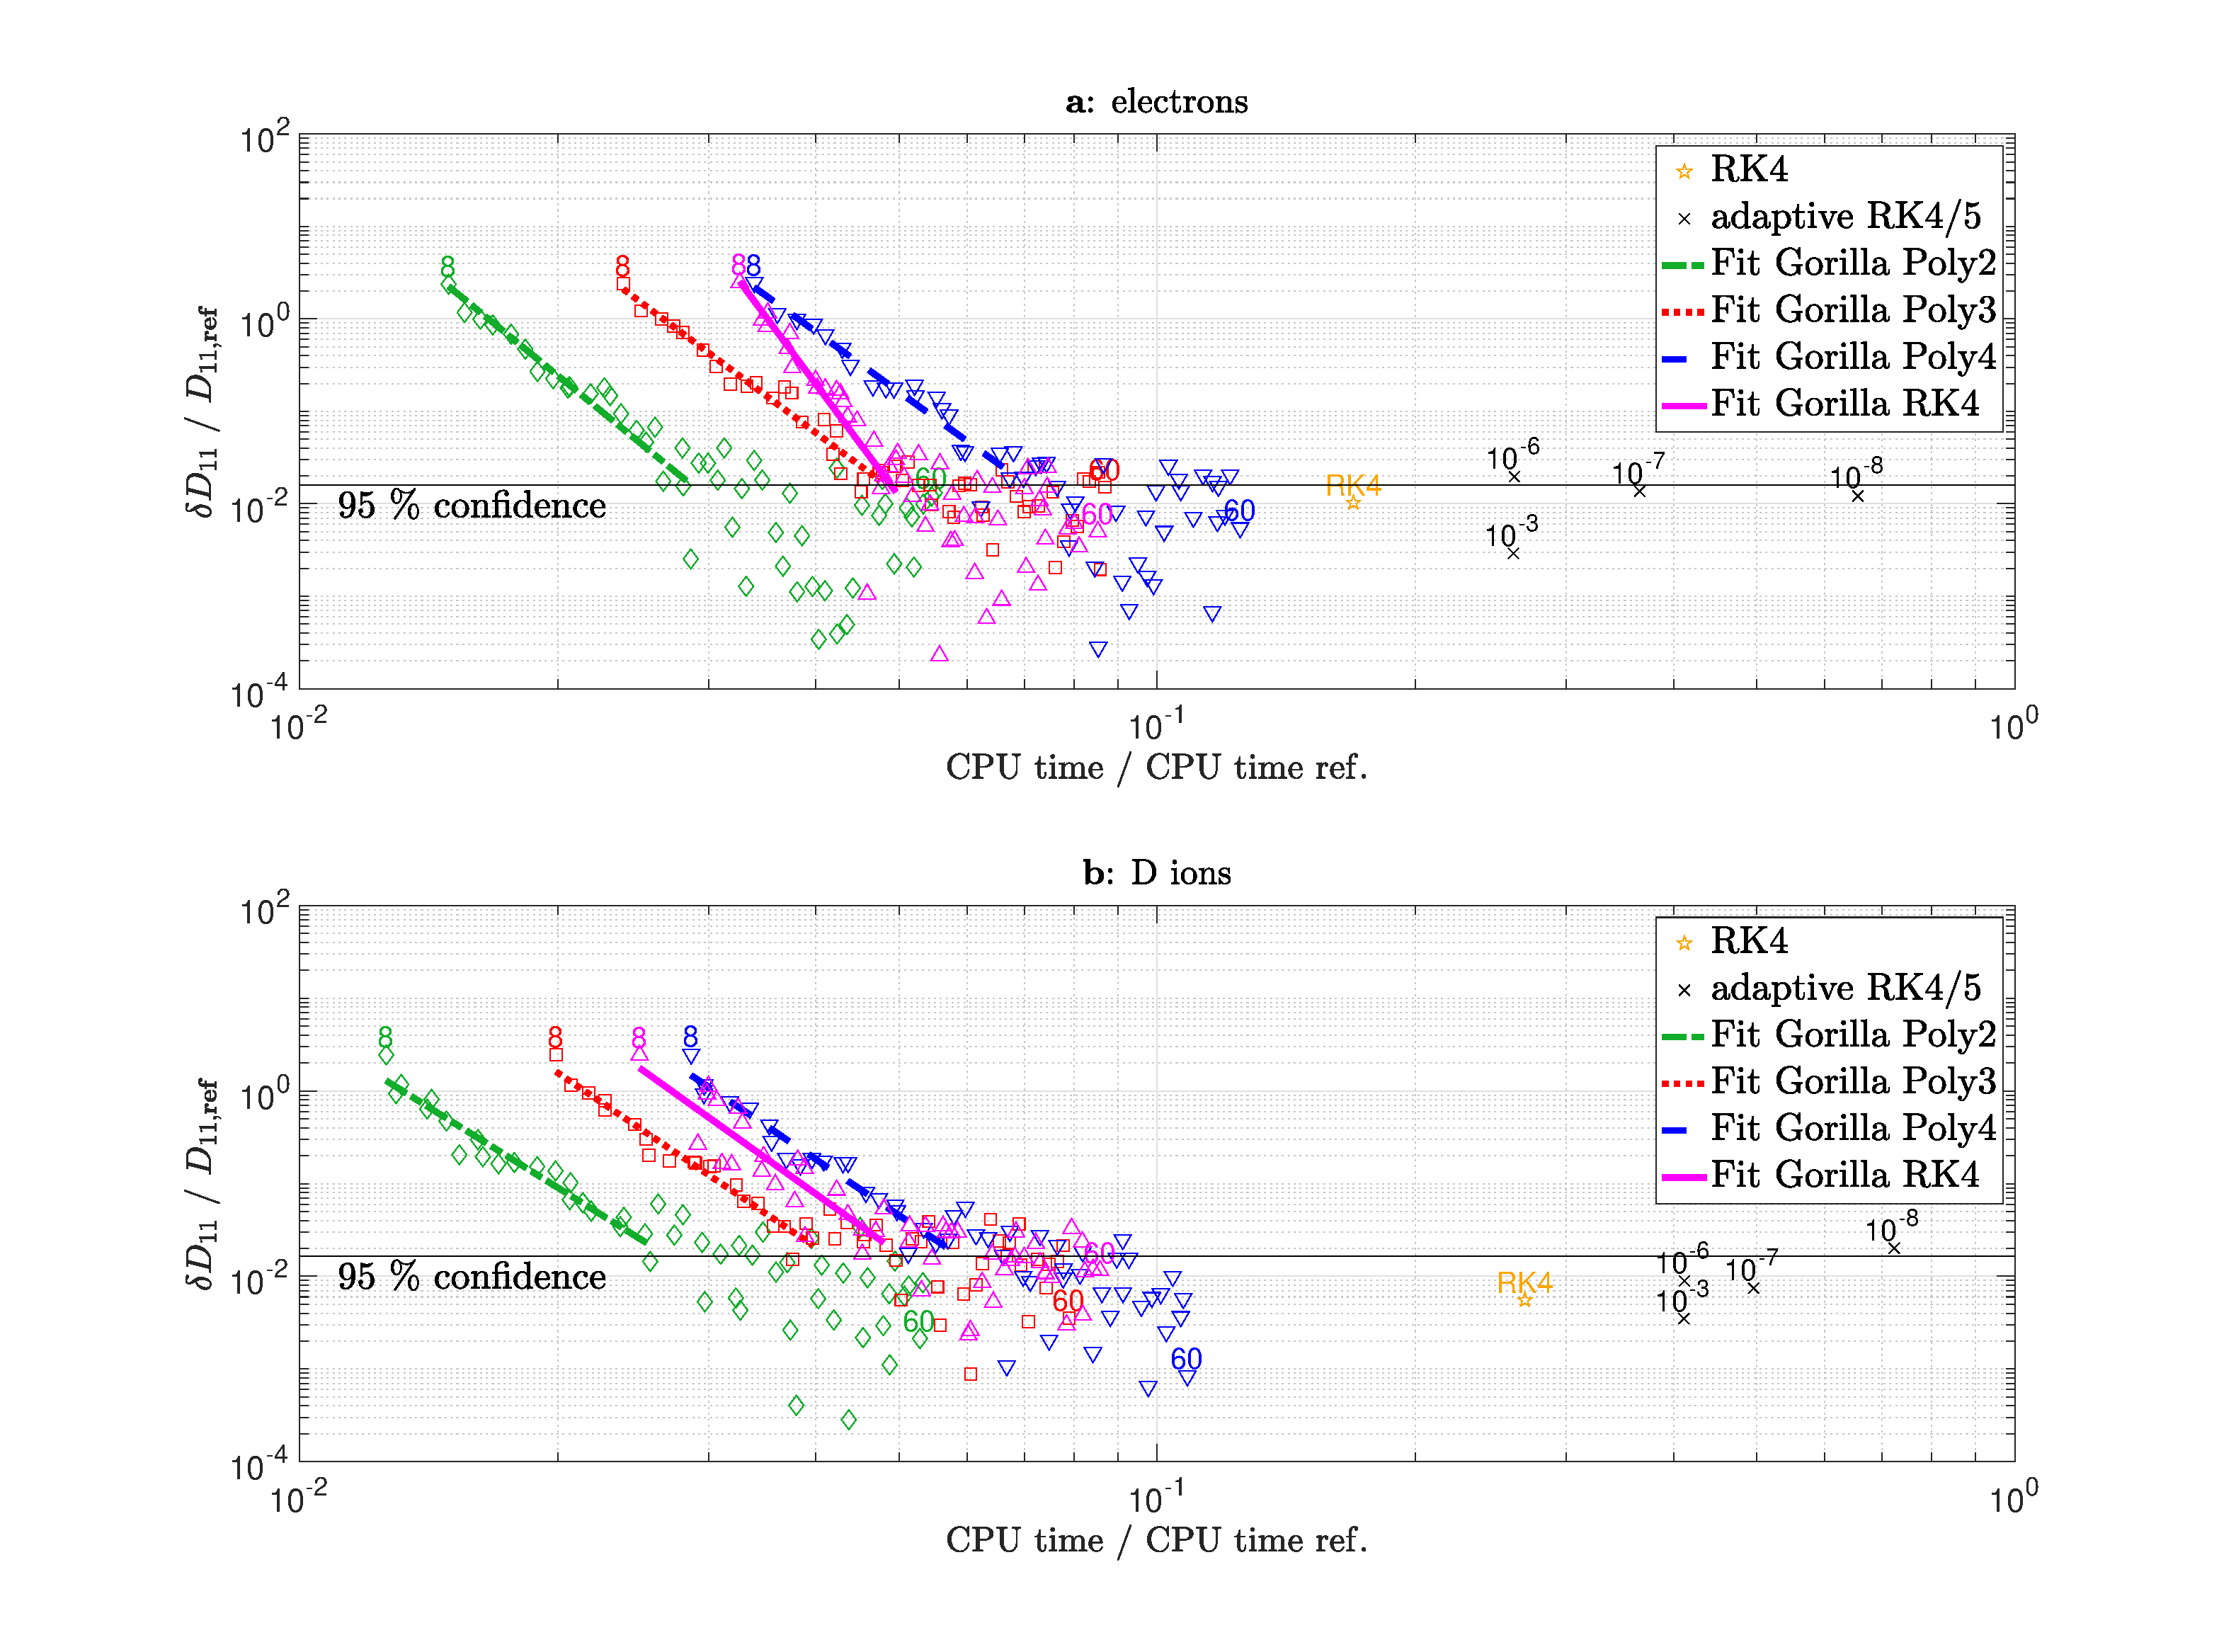
\includegraphics[keepaspectratio,width=1.1\linewidth]{figures/cpu_speed_electrons_dions.eps}}
	\captionsetup{justification=raggedright,singlelinecheck=false,textfont=footnotesize,labelfont=footnotesize}
	\caption{Relative error of mono-energetic radial transport coefficient
	$D_{11}$ of electrons (top) and D~ions (bottom) vs. relative CPU time.
	Compared orbit integration methods are:
	Runge-Kutta 4 ($\star$),
	Adaptive RK4/5 with various relative errors indicated in the plot ($\times$),
	geometric integration with polynomial solution
	(\textit{GORILLA Poly}) of the order $K=2$ ($\Diamond$), $K=3$ ($\square$) and $K=4$
	($\triangledown$), and with RK4 solution (\textit{GORILLA RK4}, $\triangle$).
	Fits of results are depicted with lines according to the legend.
	Random error of the reference result, $D_{11,\rm{ref}}$,
	is depicted as a horizontal line limiting its 95~\% confidence interval.
	}
	\label{fig:cpu_speed_electrons_dions}
\end{figure}
%
Moreover, we compare the performance and scaling for parallel computation of guiding-center orbits
using the geometric orbit integration method with
computations using standard reference integrators (RK4 and adaptive RK4/5).
For this, different integrators have been used within $D_{11}$ computation described above
for a particular choice of dimensionless parameters, $v_E^\ast = 10^{-3}$ and $\nu^\ast =  10^{-3}$,
and an increased ensemble size of $30000$ test particles.
The numerical experiment has been performed on a single node of the COBRA cluster
of MPCDF with 40 CPU cores (Intel Xeon Gold 6126) running 80 concurrent threads with hyperthreading.


The reference value for the transport coefficient, $D_{11,\rm{ref}}$,
and the reference CPU time are obtained by orbit integration
with an adaptive RK4/5 integrator with a relative tolerance of $10^{-9}$.
The accuracy of the $D_{11}$ evaluation using different computation parameter settings
is represented by the relative error $\delta D_{11} / D_{11,\rm{ref}}$
where $\delta D_{11} = |D_{11} - D_{11,\rm{ref}}|$.
The CPU time purely used for orbit integration serves as
a measure for the computational effort of the methods.
This given CPU time does not contain any overhead operations, e.g. the construction of the grid, generation of random numbers for
pitch-angle scattering and computation of $D_{11}$ by evaluating
Eq.~\ref{eq:def_d11} with the help of a least-squares regression.


Fig.~\ref{fig:cpu_speed_electrons_dions} shows the relative error of the mono-energetic
radial transport coefficient versus the relative CPU time of computations using the
geometric orbit integration
method with the polynomial series solution of various orders, \textit{GORILLA Poly},
and the iterative scheme with RK4 integration and Newton steps, \textit{GORILLA RK4}.
Accuracy and CPU time of geometric orbit integrations have been varied by
mutually changing the angular grid size $N_\vartheta \times N_\varphi$
from $8 \times 8$ to $60 \times 60$ while keeping the radial grid size
constant at $N_s = 100$. In the stellarator configuration of
Ref.~\cite{drevlak_quasi-isodynamic_2014} used here, the number of toroidal harmonic modes
per field period is $14$, leading to a minimum toroidal grid size $N_\varphi = 28$ in
order to satisfy the Nyquist-Shannon sampling theorem~\cite{nyquist_certain_1928,shannon_mathematical_1948}.
Therefore, regression lines are drawn for the range of data points with grid sizes
from $8 \times 8$ until $28 \times 28$, clearly showing a convergent behavior
of $D_{11}$ with increasing grid refinement.
Furthermore, the adaptive RK4/5 integration is additionally performed with
relative tolerances of $10^{-3}$, $10^{-6}$, $10^{-7}$ and $10^{-8}$, respectively.
Note that the computational
speed of the adaptive RK4/5 integration with a relative tolerance of $10^{-6}$ cannot be
increased by higher relative tolerances, e.g. $10^{-3}$, since the macroscopic Monte Carlo
time step, $\Delta t$ Eq.~\eq{eq:def_time_step_MC}, is already elapsed within a single
RK4/5 step with sufficient accuracy. Hence, also the non-adaptive Runge-Kutta~4 method
is tested, which naturally needs one field evaluation less per time step than RK4/5.
In all cases, the relative error of RK4/5 and Runge-Kutta~4 results is determined here
mainly by statistical deviations, with a random error dominating the bias.

Besides statistical errors due to Monte Carlo sampling, a limit for capturing
all toroidal and poloidal field harmonics is given by a minimum grid size of
two points per period due to the Nyquist–Shannon sampling theorem.
Fig.~\ref{fig:cpu_speed_electrons_dions}
visibly shows that statistical fluctuations already dominate the bias of all variants of the geometric
integration method above this sampling threshold, despite the large ensemble size of
30000 particles.
To avoid possible sampling artifacts at even higher higher particle count, we consider the geometric orbit integration method at the toroidal grid size $N_\varphi$ of
at minimum twice the number of toroidal modes in the magnetic field configurations.
The variant with the polynomial series solution truncated at $K=2$ (\textit{GORILLA Poly 2}) at
this grid resolution can be considered the fastest sufficiently accurate tested method to compute
$D_{11}$ for thermal ions and electrons. In case of D ions with an energy of 3~keV this method
is one order of magnitude faster than the Runge-Kutta~4 integrator which is the fastest
reference method.




\newpage
\end{document}